\subsection{Product Perspective}

The CLup system is expected to be developed ground-up, without any core components being shared with other services, and is expected to integrate with few external services.
The system will be using a mapping API to allow its various requirements regarding navigation.
The system will be used to control, verify, and schedule customer visits to different stores.

% Introductory text describing system's integration with other products, considering shared phenomena.

% Text for Class Diagram
% Class diagram

\begin{figure}[H]
    \centering
    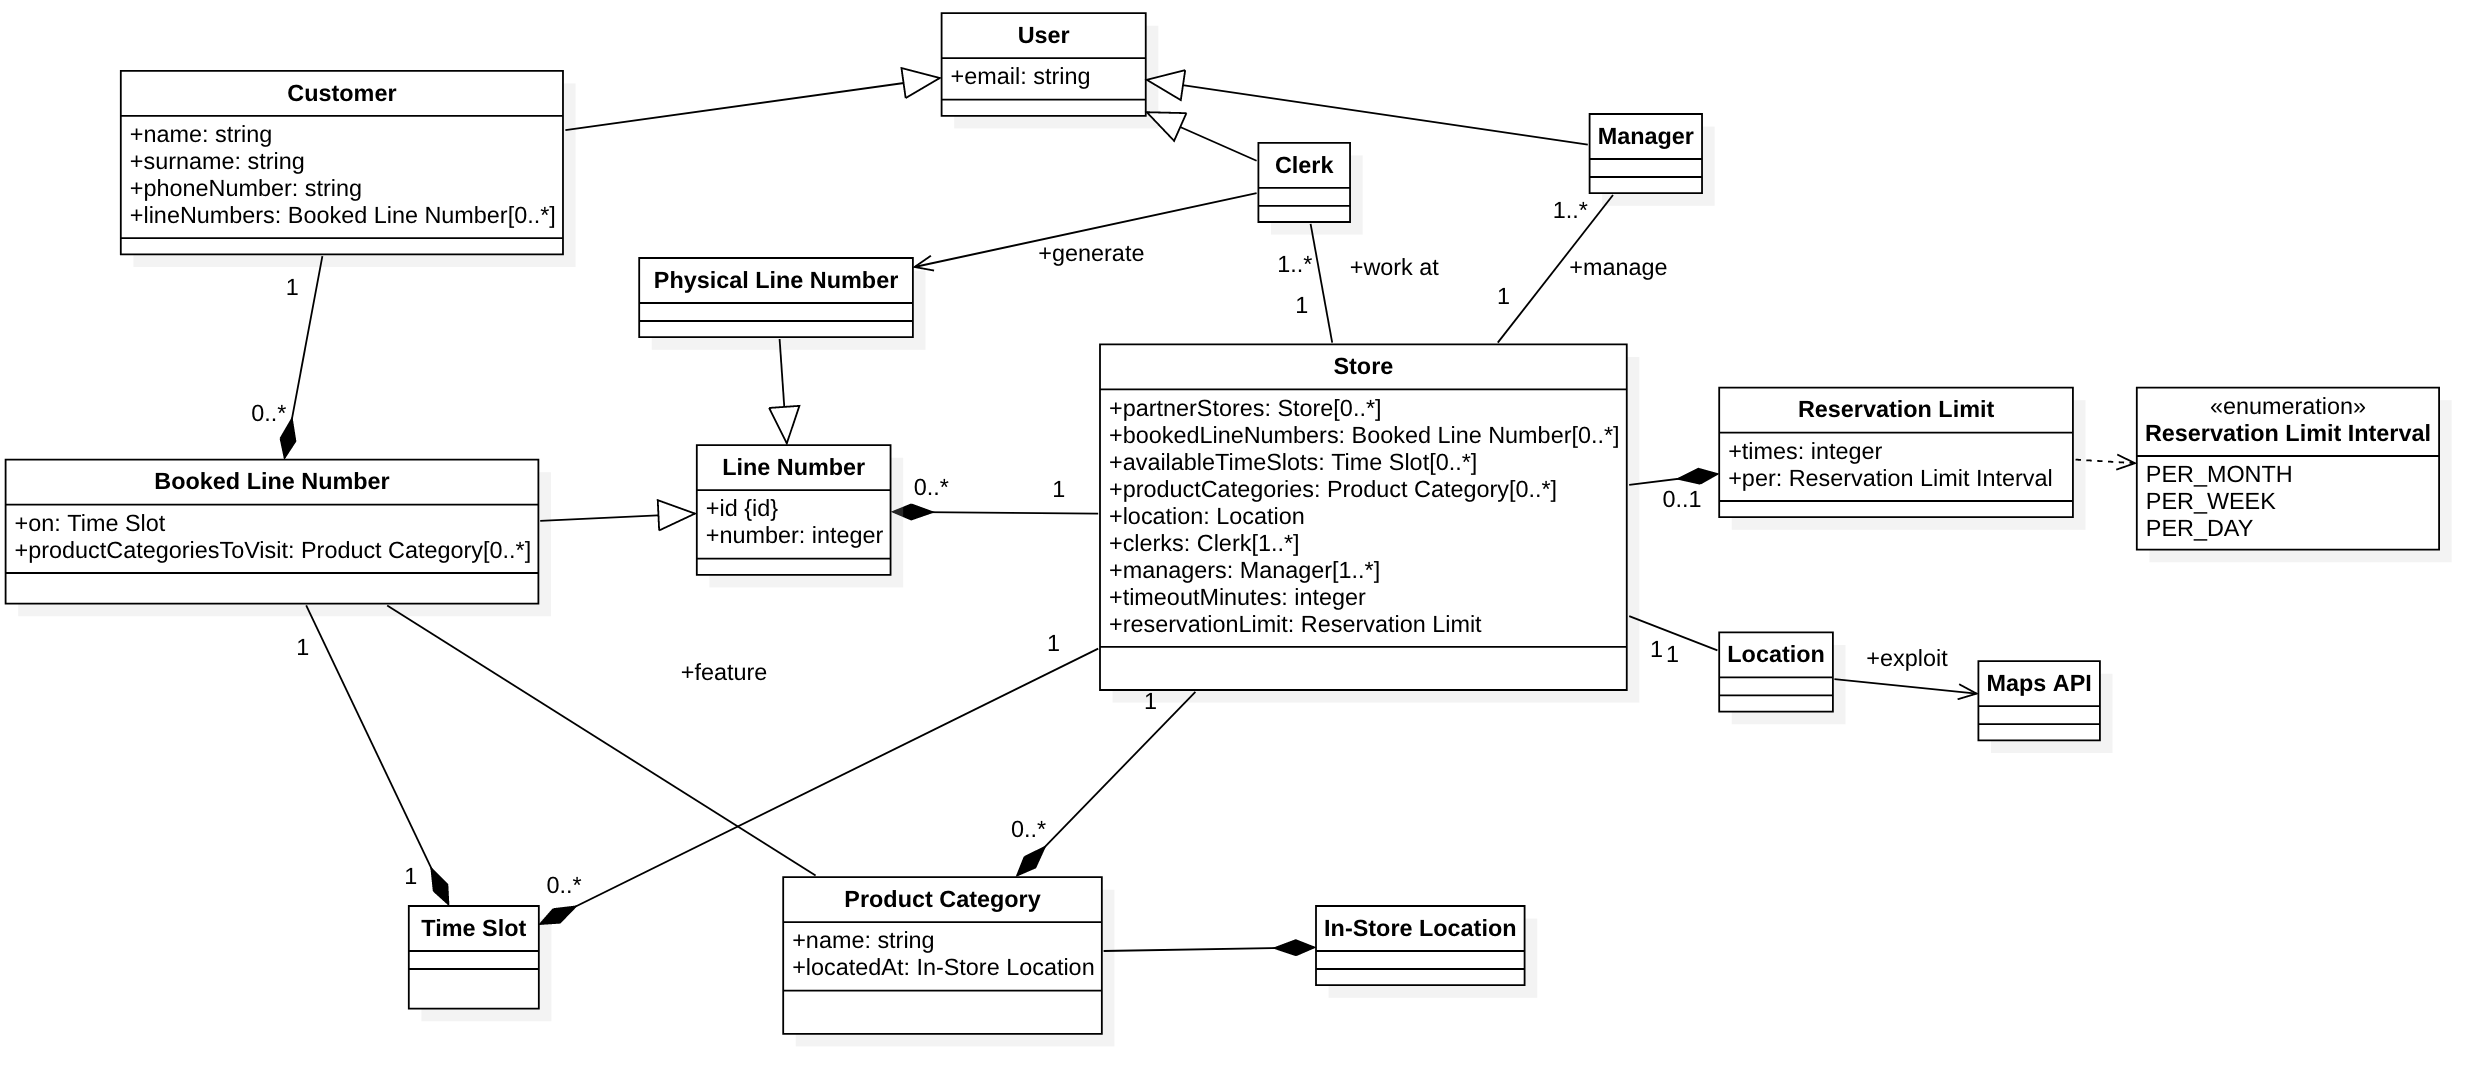
\includegraphics[height=0.5\textwidth]{Images/ClassDiagram.png}
    \caption{Class Diagram}
    \label{fig:ClassDiagram}
\end{figure}
The \nameref{fig:ClassDiagram} provided above illustrates the system's core high-level components and their interactions.


The system is designed to be used by different types of users, the \textbf{Customer}s whom visit or plan to visit the \textbf{Store}, the \textbf{Manager}s who are responsible for handling management related tasks like providing store details, handling system stops, and the \textbf{Clerk}s who are on active duty for monitoring the entrance and exit of customers.
All users on the system are identified with their \textit{e-mail}s and require their \textit{password}s to authenticate.
The \textbf{Customer}s need to register to the system with their \textit{name}, \textit{surname} and \textit{phoneNumber}, in addition to the information required for authentication.
All \textbf{Line Number}s feature a unique \textit{id} and an actual \textit{number} that indicate their order in line.
Customers can have many \textbf{Booked Line Number}s, limited by the \textit{reservationLimit}, from various stores, which provide many \textbf{Time Slot}s that the customers can select from under \textit{availableTimeSlots}, which then becomes the time slot the booking is \textit{on}.
The line number is to be invalidated after \textit{timeoutMinutes} from its target time interval.
The \textbf{Store}'s \textbf{Location} is set by the \textbf{Manager} and observed by customers through a \textbf{Maps API}.
The \textbf{Reservation Limit} imposes a customer can book a line number at most for some \textit{times} \ \textit{per} a specific \textbf{Reservation Limit Interval} (one of \textit{PER\_MONTH}, \textit{PER\_WEEK} or \textit{PER\_DAY}).
Customers' visits can also feature different \textbf{Product}s or \textbf{Product Category}ies that they might want to visit under their line number's \textit{productsToVisit} and \textit{productCategoriesToVisit}, each having a \textit{name} and \textit{locatedAt} their own \textbf{In-store Location}.
\textbf{Clerks} can generate \textbf{Physical Line Numbers} for customers that do not have the app available for them.

Below some scenarios, statecharts and their brief description are enumerated for the system's core and critical functionalities.
It is important to note that the app is targeted at users of all age ranges; thus, the scenarios feature different users of different ages.
The statecharts apply to many other scenarios that might occur out of interaction with various types of users.

% For each core feature (which are they? all?):
%   - Scenario
%   - State Chart
%   - Explanation

% Core features: Future book line number, now retrieve line number, Guest arrives to store, System stop (Shop's on fire), schedule system stop (don't forget to notify customer),
\subsubsection{Book Line Number}

\textbf{Scenario}

Ozan wants to visit the new hamburger place that has recently opened just around the corner of his house.
However, Ozan does not want to wait in a long line to purchase a burger and some fries.
The fast-food joint has incorporated the CLup system in its customer service portfolio, making it possible for Ozan to reserve his ticket beforehand without visiting the location.
Ozan downloads the CLup application and books his line number from his house.
Using the app, he can plan his route and schedule to the location beforehand and place his order directly upon his arrival.

\textbf{State Chart}

\begin{figure}[H]
    \centering
    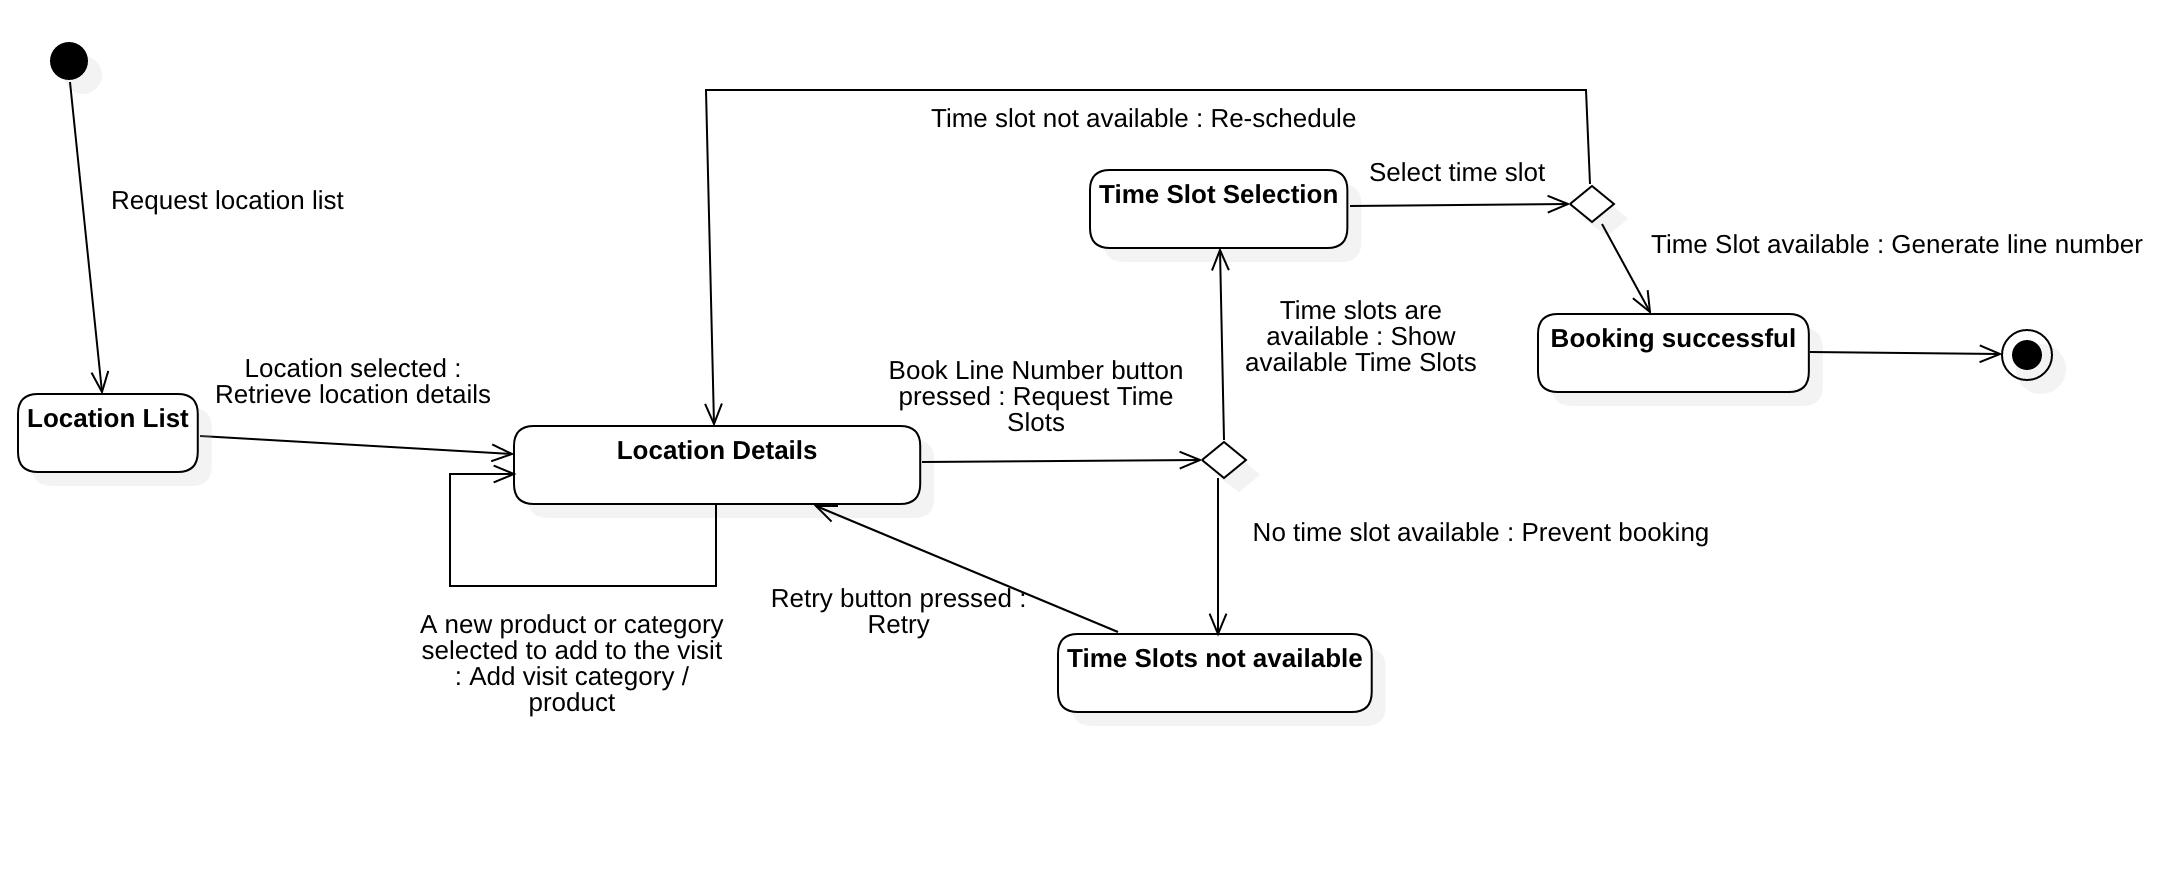
\includegraphics[height=0.4\textwidth]{Images/StateCharts/BookLineNumber.png}
    \caption{State Diagram for feature Book Line Number}
    \label{fig:SDBookLine}
\end{figure}

The \nameref{fig:SDBookLine} represents the execution flow of one of the core use cases, namely booking a line number for the future.
The customer books the line number by first listing what locations are available for them to book.
Then, when a customer selects a location, they view the location's details, where they can add products or product categories to their target visit.
The customer can then view the time slots that the system will generate specifically filtered for their visit based on the location's provided data and availability.
When the customer selects a specific time slot, the system tries to book that specific location.
If the system successfully allocates the desired time slot, it displays the success message and the customer's ticket.
Else the user is notified of the failure and brought back to the scheduling screen to select another slot.


\subsubsection{Get Line Number}

\textbf{Scenario}

Roberto lives in Milan during the COVID lockdown and wants to visit a grocery store near his house.
He wants to obtain a line number for his visit through his phone not to waste time while waiting in line for other customers to be done with their affairs.
He hears that the store he plans to visit has been on CLup, so he downloads the application and opens it.
Using the app, Roberto can now see when he should take off to reach the shop without waiting in front of the store.

\textbf{State Chart}

\begin{figure}[H]
    \centering
    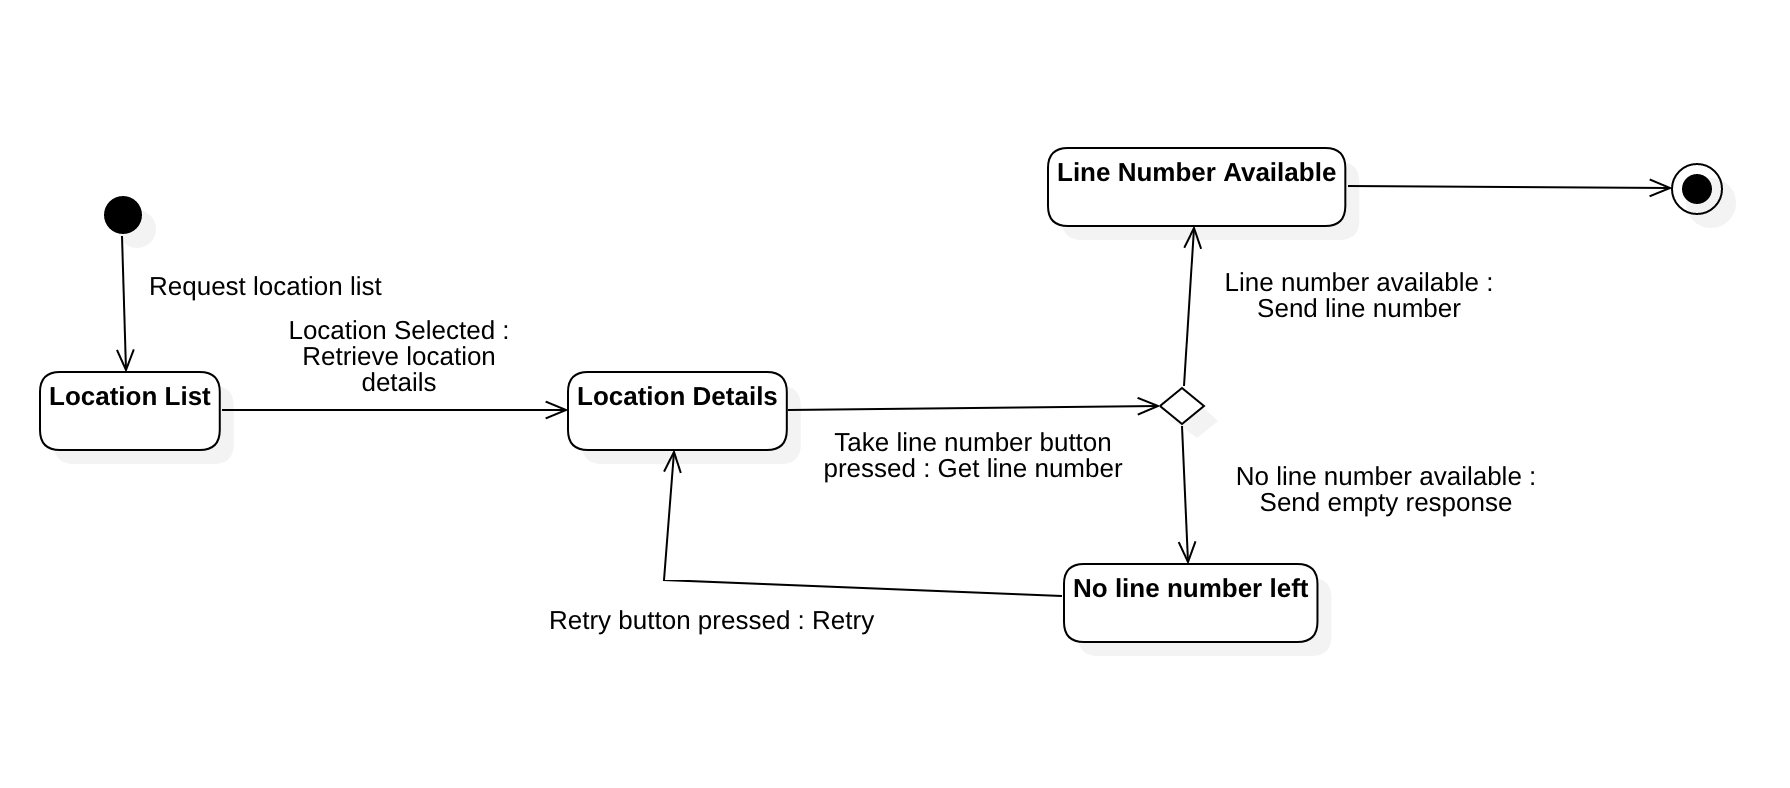
\includegraphics[height=0.4\textwidth]{Images/StateCharts/GenerateLineNumber.png}
    \caption{State Diagram for feature Get Line Number}
    \label{fig:SDGetLine}
\end{figure}

The \nameref{fig:SDGetLine} represents another core use case's execution flow, booking a line number for a recent visit.
The customer generates a line number by going over the list of available locations, similar to the Book Line Number feature; however, they press the "Take Line Number" button directly this time.
Then, the system tries to generate a line number for them, and if it is successful, the user retrieves the resulting line number.
If the system can not fulfill the user's request, it communicates the problem to the user and allows a retry.

\subsubsection{Print Line Number}

\textbf{Scenario}

Hrvoje, a Croatian who recently arrived in Italy, is not aware of the popularity of the CLup app; however, he wants to visit an electronics store to purchase a new phone because his current phone has died out of battery failure.
Upon arrival, since he does not have a phone, he can not register to the CLup system; however, the security, that is also in charge of validating line numbers, prints him a ticket that he should keep during his whole visit.
Therefore, Hrvoje is allowed in the store, even if he does not have the application, and the shop manager can monitor his entrance and exit.

\textbf{State Chart}

\begin{figure}[H]
    \centering
    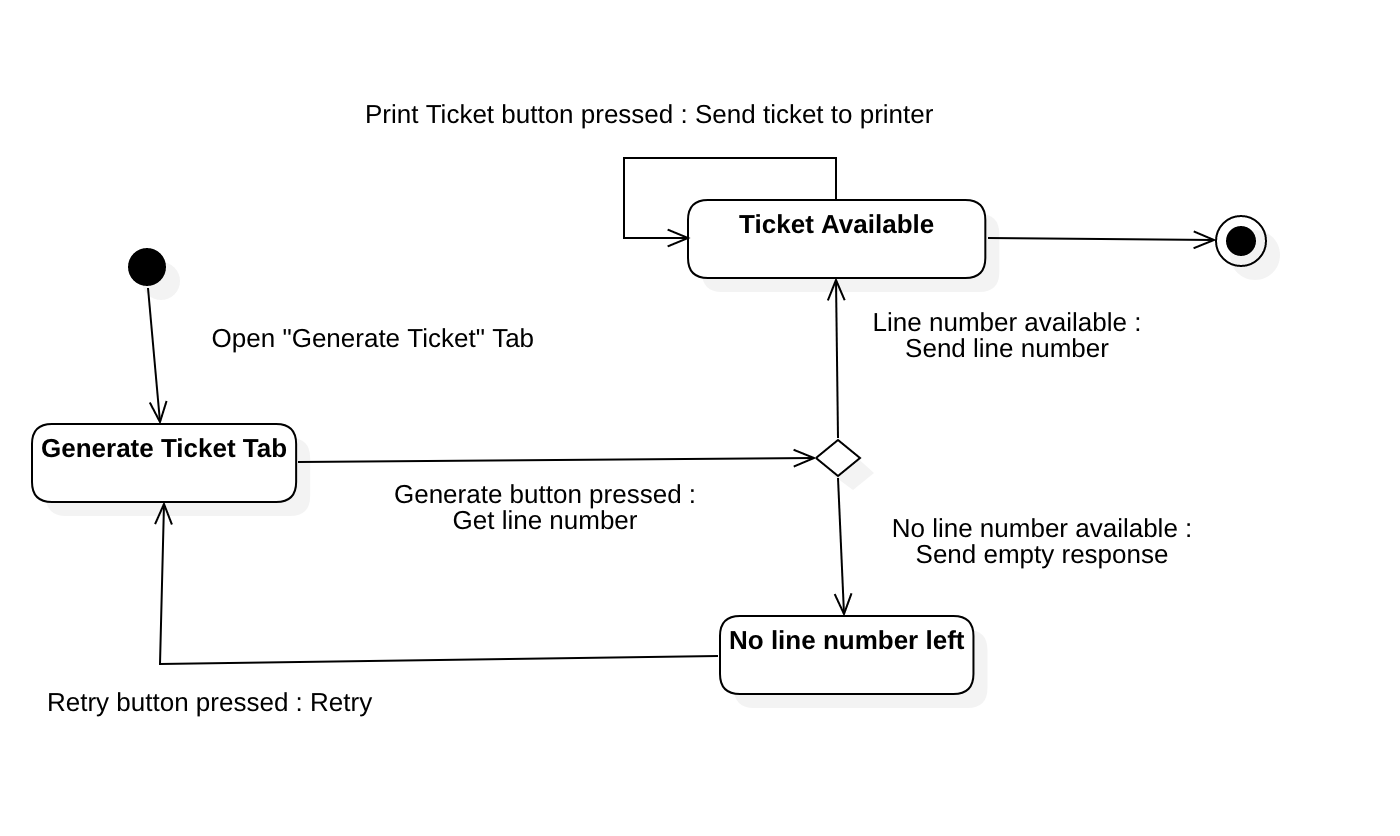
\includegraphics[height=0.4\textwidth]{Images/StateCharts/PrintTicket.png}
    \caption{State Diagram for feature Print Line Number}
    \label{fig:SDPrintLine}
\end{figure}

The \nameref{fig:SDPrintLine} represents the execution flow of a similar use case, printing an actual ticket for on foot visitors.
Upon the arrival of a new customer that does not have a line number, the clerk opens the generate ticket tab and presses the "Generate" button to create a new line number.
If all the constraints are satisfied, the system allocates a new ticket number for the customer.
The clerk can then print the ticket out using a printer.
In case there are no line numbers left, the system notifies the clerk as such, with an option to retry the operation.

\subsubsection{System Stop}

\textbf{Scenario}

Gianfranco is a team lead in a shoe factory.
The shoe factory also has an outlet store, where the local brand sells its shoes directly to customers at a discounted price.
One day, a fire erupts due to a malfunction in the automated sewing machine, and it starts to spread all over the building.
Gianfranco coordinates the evacuation of the factory and the store.
He also uses the CLup application to issue a system stop to prevent further customers from flooding in.
All the store customers receive notification regarding this unfortunate event and do not arrive at the location.

\textbf{State Chart}

\begin{figure}[H]
    \centering
    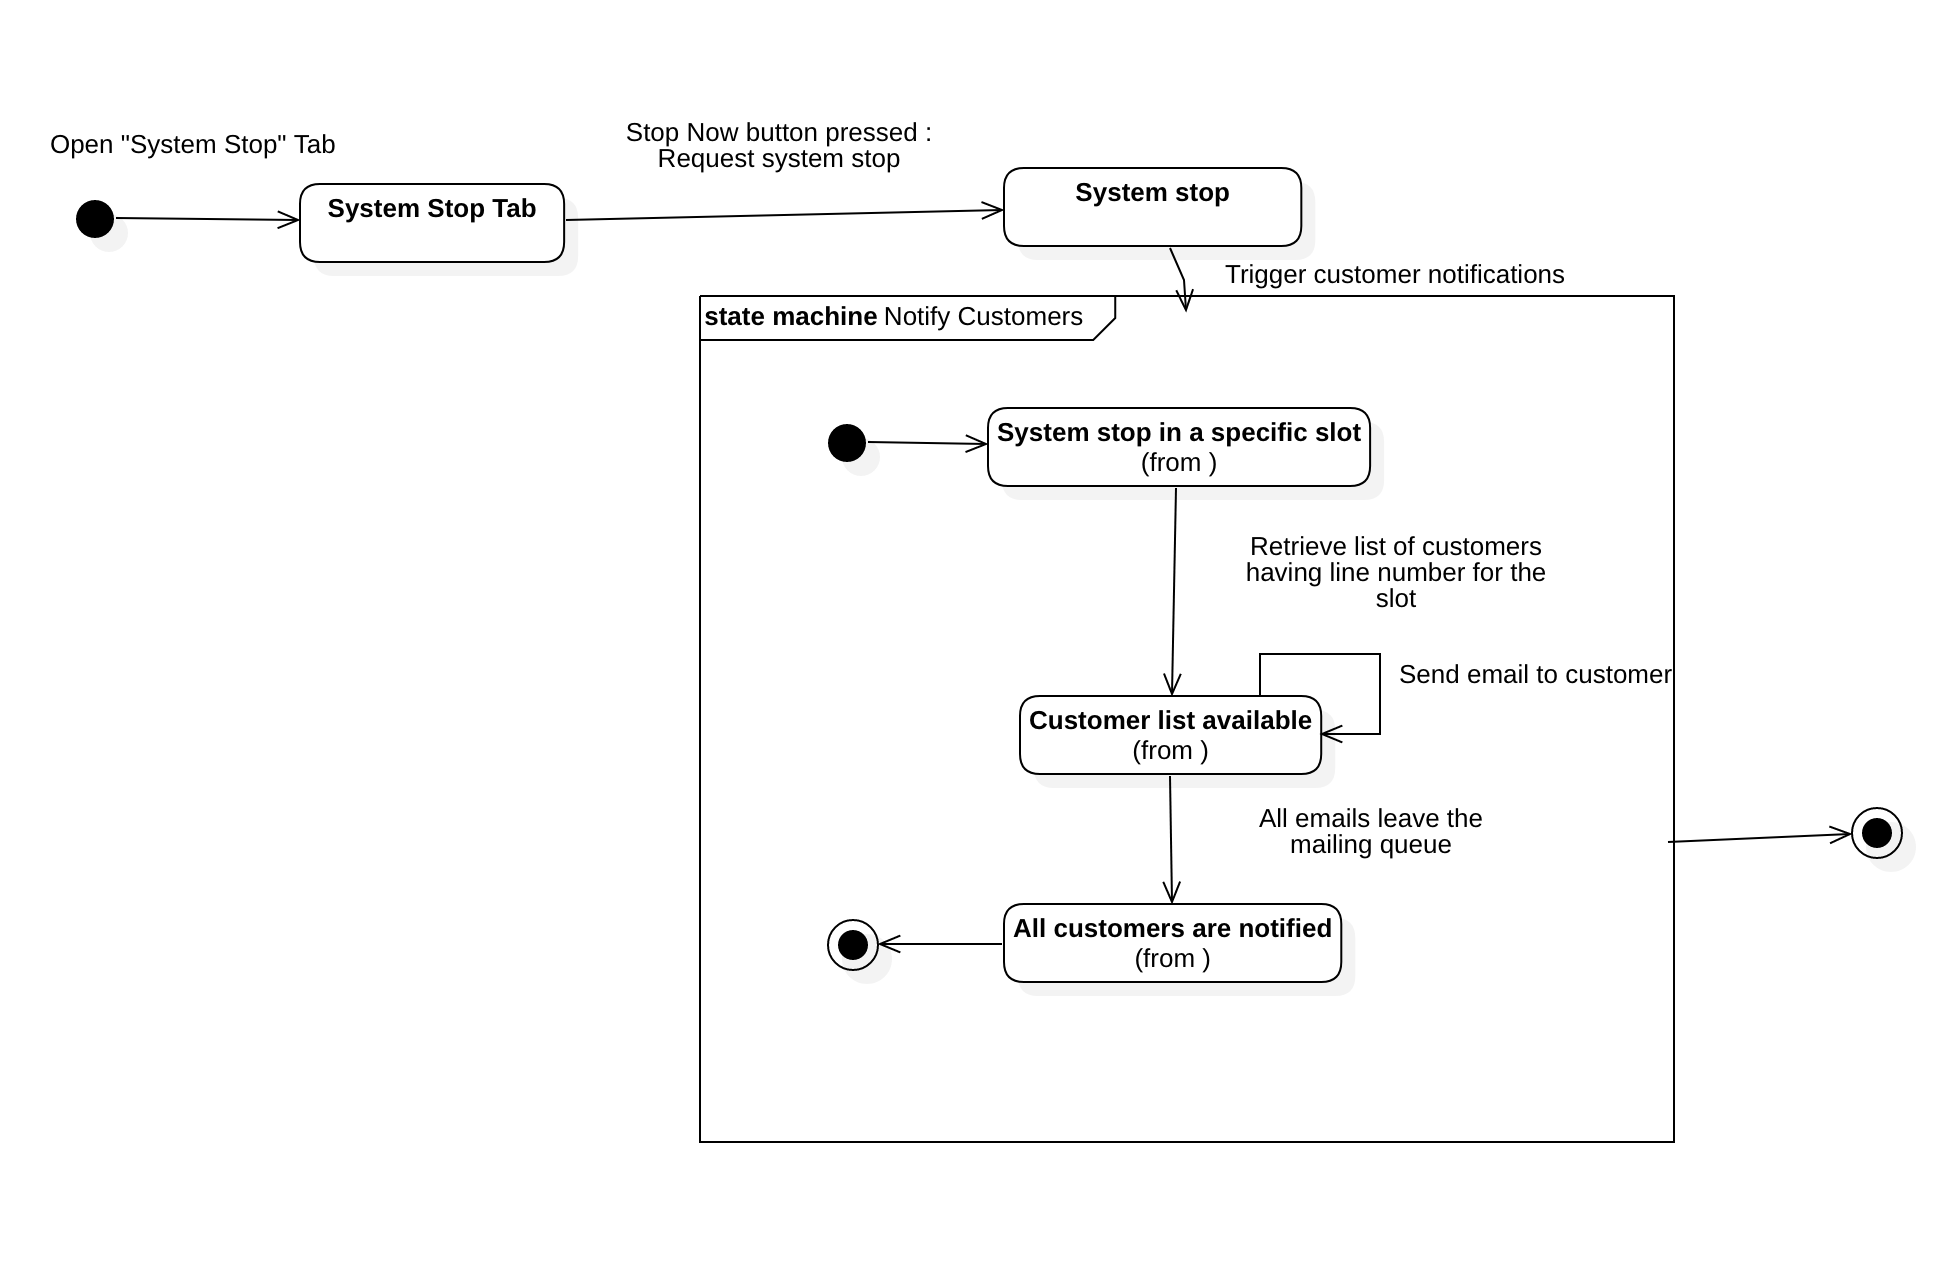
\includegraphics[height=0.4\textwidth]{Images/StateCharts/SystemStop.png}
    \caption{State Diagram for feature System Stop}
    \label{fig:SDSystemStop}
\end{figure}

The \nameref{fig:SDSystemStop} represents the execution flow for a critical use case, the manager's ability to halt the system so that all line numbers get canceled, all users are notified, and no other line numbers are issued.
The manager first opens the System Stop tab on their phone and afterward requests a system stop.
This action stops the system from issuing more tickets and triggers the distribution of notifications for the time zones the system is stopped in.
In the notification part of the state diagram, the system starts with a request for a stop for a specific time slot and retrieves all the customers that have already scheduled for that slot.
The system then starts sending emails to all customers that are in the list provided.
When all emails leave the mailing queue, the system has successfully notified all the customers regarding the stop.
The state machine of Notifying Customers is re-used to describe the notification mechanism in the \nameref{fig:SDScheduleStop}.

\subsubsection{Schedule System Stop}

\textbf{Scenario}

Giuseppe is the owner of a famous local pizza place.
He is using the CLup system in his store to manage the customer lines.
He is also preparing a new radio advertisement for his store, with an advertisement agency.
They have a meeting next week during work hours, and he does not have anyone to give the authority to manage the store.
Therefore, he has to shut the store down for half the day.
He schedules a system stop from the CLup system to prevent ticket numbers from being issued on that day for his store.

\textbf{State Chart}

\begin{figure}[H]
    \centering
    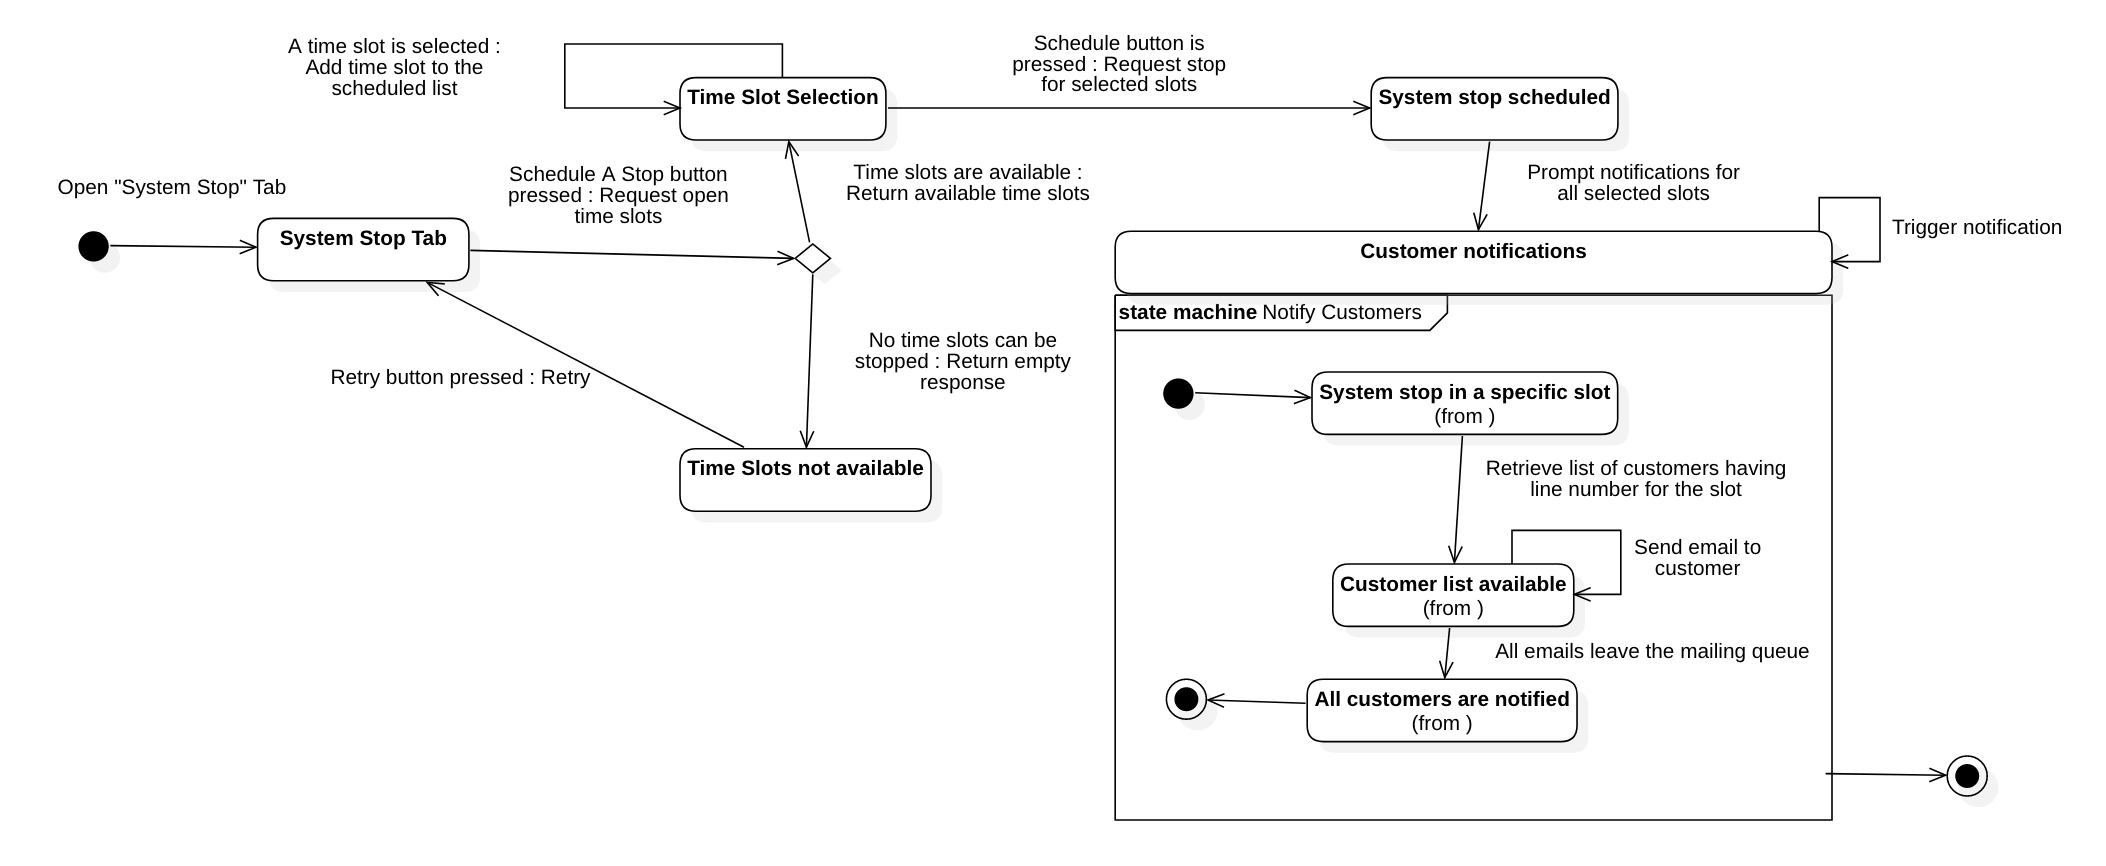
\includegraphics[height=0.4\textwidth]{Images/StateCharts/ScheduleSystemStop.png}
    \caption{State Diagram for feature Schedule System Stop}
    \label{fig:SDScheduleStop}
\end{figure}

The \nameref{fig:SDScheduleStop} represents the final core use case of the system that is considered significant, scheduling the system to stop in the future.
To start this flow, the manager first opens the System Stop tab and presses the schedule a stop button.
The system then pools all the available slots that the manager can issue a stop on and returns the list to the time slot selection screen.
If no such slot is available, a screen indicating such a case is visible, with an opportunity to retry the action.
The manager selects specific time slots from the time slot selection list that the system shall stop for and press the Schedule button to schedule a system stop.
A scheduled system stop also sends a notification to all customers that have booked a time slot for that shop before the system stop.
The mechanism of customer notification is detailed in the description of the \nameref{fig:SDSystemStop}, so it will not be repeated here.
% here  we  include scenarios  and further details on the shared phenomena and a domain model (class diagrams and state charts)


\subsection{Product functions}
% TODO: @Hrvoje do these 3

% subsubsections with functions of (some?) requirements
% here we include the most important requirements
% for requirements use the R_1, R_2, R_3 syntax


\subsection{User characteristics}
% User roles: Manager & User & Clerk (& maybe unregistered user?)

% People need to be able to use Tickets, maybe: %90 / %10
% here we include anything that is relevant to clarify their needs


\subsection{Assumptions,dependencies and constraints}
\subsubsection{Domain Assumptions}

\begin{itemize}
    \item \textbf{$D_1$} \%80 of the customers and all clerks and managers have basic ICT skills, has an e-mail address that they are willing to use to authenticate to the system, and has a smartphone or equivalent device that can connect to the Internet, have a browser that supports UTF-8, display QR codes and has a mapping application.
    \item \textbf{$D_2$} Locations will be visited by no more than 1000 people in any time slot.
    \item \textbf{$D_3$} \%98 of the customers will arrive at the given location either without a ticket or with a ticket that has not timed out.
    \item \textbf{$D_4$} E-mail addresses are not shared by multiple users of the system.
    \item \textbf{$D_5$} Clerks' mobile devices are equipped with at least one camera that the system can use.
    \item \textbf{$D_6$} All users have a basic understanding of how the line numbering system works and respects the system's ordering.
    \item \textbf{$D_7$} Managers have an estimate for the number of reservations that their location can at most have.
    \item \textbf{$D_8$} Managers' device has location services with a location acquisition error for no more than 20 meters.
    \item \textbf{$D_9$} Clerks are continually monitoring the locations entrances and exits.
    \item \textbf{$D_{10}$} Locations have printing equipment in 5 meters range of all the entrances that can print QR codes and line numbers.
    \item \textbf{$D_{11}$} At least one manager is available in the location during the working hours.
    \item \textbf{$D_{12}$} The customer's entry and exit to the store are determined by whether the clerks have checked them in and out.
    \item \textbf{$D_{13}$} The customer has their line number or line number ticket available with them through their visit, including their exit from the store
\end{itemize}

% here we include domain assumptions
% use the D_1, D_2,... syntax
\subsubsection{Dependencies}
% TODO: @Hrvoje these 2 too.
% Maps API
% What external libraries, tools, integrations does the system rely on
\subsubsection{Constraints}
% Maps API failure
% All user and location info can be represented with UTF-8 character encoding.
% What are the limits imposed by the environment, regulatory policies, hardware & software limitations, etc...
